O problema de decisão \textit{Grape Puzzle} consiste na resolução de \textit{n-1}+...+1 somas, em que as cores representam variáveis iguais. Tomemos o exemplo, do problema seguinte, com 4 linhas:
\begin{figure}
    \centering
    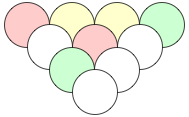
\includegraphics{problem.png}
    \caption{Problema de 4 Linhas}
    \label{fig: 4rowproblem}
\end{figure}

As somas correspondentes, apresentadas de linha a linha, serão:

\begin{equation}
    \systeme*{
    A \+ B = D  &\bigcap B \+ B = A  &\bigcap B \+ C = E ,
    D \+ A = C &\bigcap A \+ E = F,
    C \+ F = G
    }
\end{equation}

Tendo como solução:
\begin{figure}
    \centering
    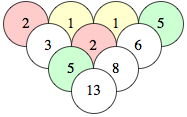
\includegraphics{solution.png}
    \caption{Solução de um problema de 4 Linhas}
    \label{fig: 4rowsolution}
\end{figure}